\documentclass[12pt]{article}
\usepackage{float}
\usepackage[margin=0.8in]{geometry}
\usepackage[utf8]{inputenc}
\usepackage[fleqn]{amsmath}
\usepackage{times}
\usepackage{hyperref}
\usepackage{multirow}
\usepackage{graphicx}
\usepackage{mathptmx}
\usepackage{caption}
\usepackage{csquotes}
\usepackage[font=scriptsize,labelfont=bf]{caption}
\graphicspath{{./img/}}

\title{CS3211 Project 2: OthelloX}
\author{Tan Soon Jin, A0112213E \\ a0112213@u.nus.edu}
\date{\today}

\begin{document}
\maketitle

%%%%%%%%%%%%%%%%%%%%%%%%%%%%%%%%%%%%%%%%%%%%%%%%%%%%%%%%%%%%%%%%%%%%%%%%%%%%%%%%%%%%%%%%%%%%%%%%%%%%

\section{Introduction}

To generate the best move for a game of othello, I have implemented a \textbf{minimax
with alpha-beta pruning} as the sequential game tree search algorithm. In
addition, some enhancements are made such as using \textbf{transposition table} to store
best moves for a particular board configuration and \textbf{killer heuristic} to
consider more promising move first.

I have experimented with 2 board representations: the first being a \textbf{1D array} to
store the board configuration which is more efficient than a 2D array because of
data locality. Secondly, \textbf{bitboard} which is a bit array data stucture
that is commonly used in board game is also implemented. Leveraging on bitwise
operations which can be done in parallel, faster move generation and board
evaluation can be achieved.

For the parallelization of game tree search, this paper primarily look at
\textbf{Principle Variation Split}, \textbf{Young Brother Wait Concept} and
\textbf{Dynamic Tree Splitting}. The paper will further elaborate on the
strategies used to achieve optimal \textit{load balancing},
\textit{communication / computation ratio} and \textit{aggregation of tasks}.



%%%%%%%%%%%%%%%%%%%%%%%%%%%%%%%%%%%%%%%%%%%%%%%%%%%%%%%%%%%%%%%%%%%%%%%%%%%%%%%%%%%%%%%%%%%%%%%%%%%%

\section{Sequential game tree search}

\subsection{Minimax game tree search}

\begin{figure}[H]
  \centering
  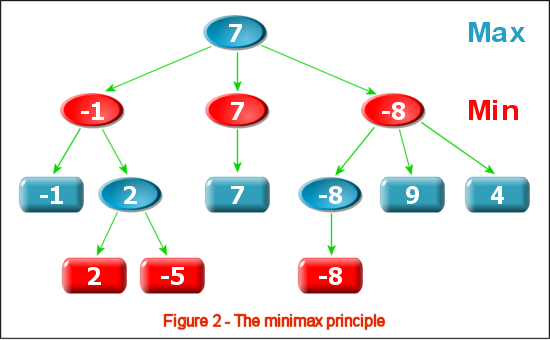
\includegraphics[width=0.5\textwidth, height=0.3\textwidth]{minimax.png}
  \caption{Minimax game tree. \href{}{http://www.hamedahmadi.com/gametree/minimax6.png}}
  \label{fig:minimax}
\end{figure}

Looking into various computer games like chess, checker and otheelo, minimax
algorithm is the standard solver which is easy to implement and generates
relatively good result. Minimax algorithm effectively is trying to minimize the
possible loss for the worst case scenario with the assumption that the opponent
will take the most optimal move. As show in Figure \ref{fig:minimax}, it works by first
generating all possible moves at an increasing depth with a depth-first search
strategy.

\begin{figure}[H]
  \centering
  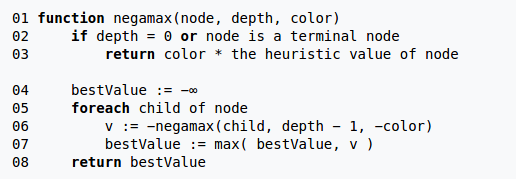
\includegraphics[width=0.4\textwidth, height=0.2\textwidth]{negamax.png}
  \caption{Negamax: simplified variant of minimax}
  \label{fig:negamax}
\end{figure}

For this project, negamax which takes advantage of the relationship $max(a,b) =
min(-a, -b)$ which reduces to one subroutine instead of 2 subroutines for the
original minimax approach. With this each evaluation is performed with respect
to the current player's point of view. Provided in Figure \ref{fig:negamax} is a simple pseudocode for negamax:

\subsection{Alpha-beta pruning}

\begin{figure}[H]
  \centering
  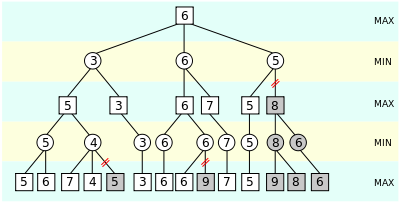
\includegraphics[width=0.5\textwidth, height=0.3\textwidth]{alphabetapruning.png}
  \caption{Alpha-beta pruning: greyed out nodes are pruned}
  \label{fig:alphabeta}
\end{figure}

Alpha-beta pruning is an optimization on the common minimax algorithm that
prunes the search tree by removing subtrees of moves which will definitely not
be searched. It works as shown in Figure \ref{fig:alphabeta} by maintaining an
$\alpha$: maximum lower bound and $\beta$: minimum upper bound. Any node in the
search tree that does not fall between these bounds will be pruned, and thus reducing the search space.  

\subsection{Alpha-beta enhancement}

\subsubsection{Transposition table}

\textit{Transposition table} is a large hash table that stores results of
previously performed searches. During a search, the program may encounter the
same board configuration in different subtrees (this is known as transposition).
Inspired by dynamic programming  paradigm, this approach greatly reduces search
space of the program by removing redundant search.

In our hash table, the score, alpha value, beta value and depth of tree is
stored. \textit{Zobrist hashing} is used to generate the hash of the table. In a
parallel environment, usage of lock is inevitable for synchronization of data.
However, usage of lock is detrimental increases the \textit{synchronization
  overhead} when the number of processor increases.

To solve this problem, this paper follow the approach of
\cite{rasmussen2004parallel} of storing the XOR of hash key with the board
state. If a corruption is detected, the value is recalculated. Another approach
is to use a coarse-grain lock on the transposition table, where multiple entries
of the table share a same lock to reduce the overhead of using a locking mechanism.

There are 2 advantages of using a transposition table: 1) reduce the search
space of game tree and 2) move ordering based on previous searches which is
essential for alpha-beta pruning.


\subsubsection{Killer heuristic}

\textit{Killer heuristic} works by storing N moves that generated a cutoff for a
particular depth. This works under the assumption that the \textit{killer moves}
may generate a cutoff in the current position.

\subsection{Evaluation function}

I propose a linear combination of piece differential, mobility potential and
stability potential as the evaluation function for the otheelo program.
Generating a sophisticated can be time consuming and requires a lot of machine
learning which is out of the scope of the project. Below is brief description of
the implemented evaluation function:

\begin{enumerate}
  \item \textbf{Piece differential} \\
    score = number of discs - number of opponent's discs
  \item \textbf{Current mobility} \\
    score = number of legal moves - number of opponent's legal moves
  \item \textbf{Frontier mobility} \\
    score = number of discs with empty squares in all direction - number of
    opponent's discs with empty squares in all direction
  \item \textbf{Stability} \\
    score = number of discs that cannot be flipped - number of opponent's
    discs that cannot be flipped
\end{enumerate}

%%%%%%%%%%%%%%%%%%%%%%%%%%%%%%%%%%%%%%%%%%%%%%%%%%%%%%%%%%%%%%%%%%%%%%%%%%%%%%%%%%%%%%%%%%%%%%%%%%%%

\section{Board representation}

\subsubsection{Bitboard}

Each board state is stored as bit array with one or more \textit{uint64}
because the board dimension is not fixed. Bitboard approach is both compact and
allow for faster evaluation and move generation. These steps that are performed
by each node could benefit massively from usage of bitwise operations that
consequently reduces the search time of the program.

Using various filters or masks, generation of legal moves can be achieved easily
as shown in Figure \ref{fig:bitboard_legalmoves}. Legal moves in Othello
consists of moves that can capture a line of opponent's discs.

\begin{figure}[H]
  \centering
  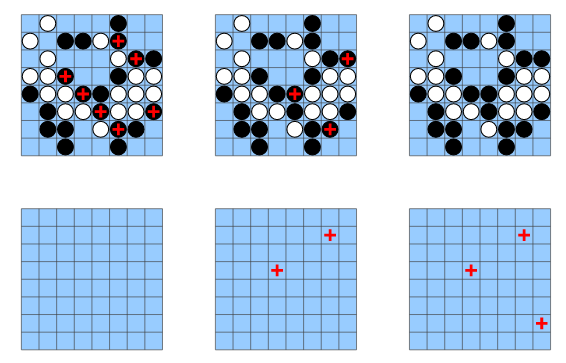
\includegraphics[width=0.5\textwidth, height=0.3\textwidth]{bitboard_legalmoves.png}
  \caption{Top: line propagation, Bot: legal moves}
  \label{fig:bitboard_legalmoves}
\end{figure}

\subsubsection{1D array}

Though bitboard is perfect for move generation and evaluation, it can be slow
for query such as what type of disc (black or white) is present at a particular
position. Therefore, a 1D array is used to store positions of disc for both players.


%%%%%%%%%%%%%%%%%%%%%%%%%%%%%%%%%%%%%%%%%%%%%%%%%%%%%%%%%%%%%%%%%%%%%%%%%%%%%%%%%%%%%%%%%%%%%%%%%%%%
\section{Parallel Game Tree Search}

\subsection{Naive Parallel Alpha-Beta}

The first approach to parallelize alpha beta pruning involve splitting legal
moves at depth = 1 to each available processors. Consequently, we try splitting
the subtrees at deeper depth which causes higher workload imbalance as the lack
of information from other trees disallows for pruning to be done.
Tree-decomposition at width means each processor can be assigned different
possible legal moves.

\subsubsection{Tree-decomposition models}

\begin{figure}[H]
  \centering
  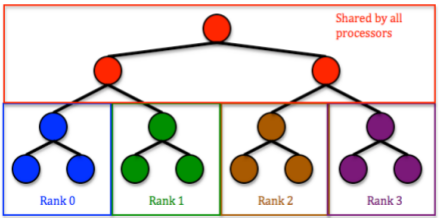
\includegraphics[width=0.5\textwidth, height=0.3\textwidth]{parallel_depth.png}
  \caption{Even-split model for tree-decomposition}
  \label{fig:parallel_depth}
\end{figure}

\textbf{Even split model} splits n children among p processors for processing
independently. \textit{MPI\_GATHER} is used to aggregate best result from each
processor to process 0. The process will then broadcasts the best results to the
other processes. An example of how the decomposition is performed can be seen in
Figure \ref{fig:parallel_depth}

The \textbf{master-slave} model on the hand explores \enquote{manager-worker} and \enquote{asynchronous
  iteration} paradigms. The \textbf{manager} process is responsible
for:

\begin{enumerate}
  \item distibutes evaluation of a particular legal move to a worker process
  \item gathers the best cost functions and values returned by the worker
    processes using \textit{MPI\_GATHER}
  \item determines best evaluation function value using \textit{MPI\_REDUCE}
  \item broadcasts the best move so far to worker processes using \textit{MPI\_Bcast}
\end{enumerate}


\noindent The \textbf{worker} process on the hand has to:
 
\begin{enumerate}
  \item Evaluates a board state assigned by manager process
  \item Sends the score and best move to manager process
  \item Receives designated move from manager process
\end{enumerate}


\noindent With this approach we are still missing the benefit of pruning as the
best alpha beta bounds are only found at deeper depths.


\subsubsection{Evaluation}

\begin{figure}[H]
  \centering
  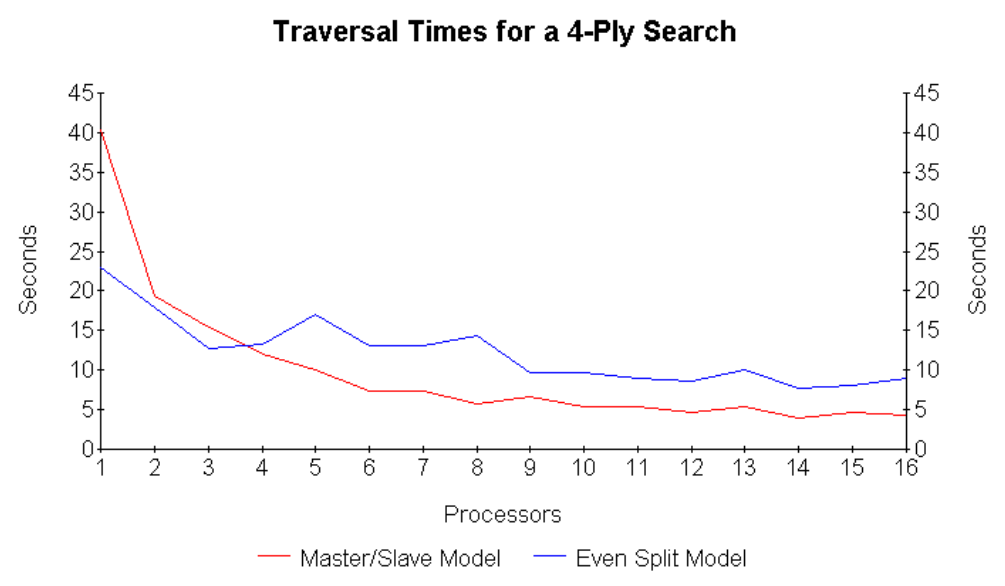
\includegraphics[width=0.6\textwidth, height=0.4\textwidth]{traversal_model.png}
  \caption{Comparing traversal time for master-slave model and even-split model}
  \label{fig:traversal_model}
\end{figure}

As we can see in Figure \ref{fig:traversal_model}, master-slave model has a
shorter traversal time compared to the even-split model for lower number of processors.

\begin{figure}[H]
  \centering
  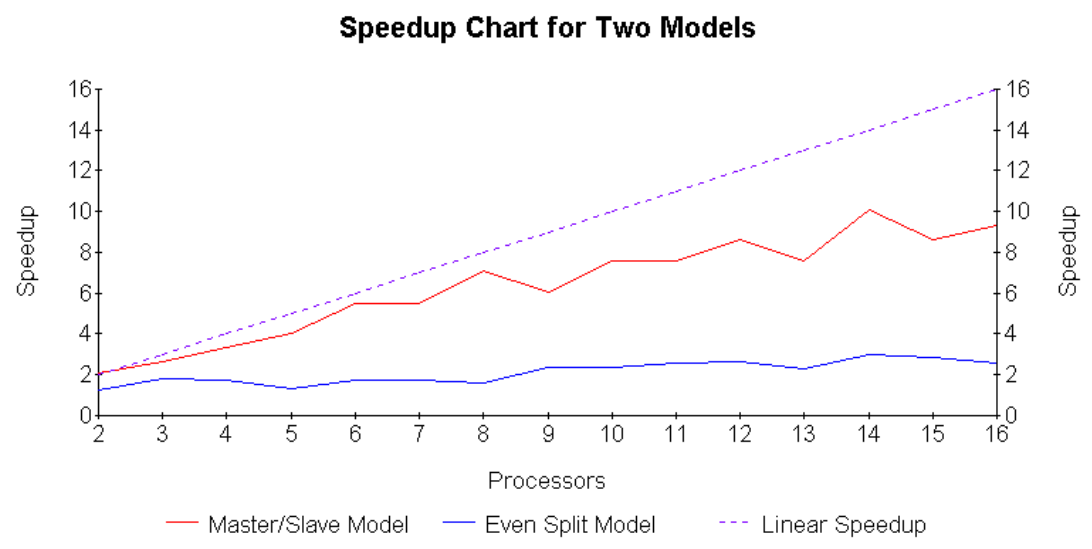
\includegraphics[width=0.6\textwidth, height=0.4\textwidth]{speedup_model.png}
  \caption{Comparing speedup for master-slave model and even-split model}
  \label{fig:speedup_model}
\end{figure}

From Figure \ref{fig:speedup_model} that compares the speedup of the even-split
model and master-slave model, the master-slave model outperforms the even-split
model in terms speedup and efficiency. It showed an almost linear speedup which
can be attributed to pre-assigning processors to subtrees prevent the program
from making full use of all the processors. Some processors that have completed
their work have to wait for completion of other processors.



\subsection{Combining OpenMP \& MPI}

In addition, this paper also explores a hybrid approach of OpenMP for
thread-management and MPI that see a lot of application in recent years. In this
section, we will look at brief overview of this approach and its benefits:

\subsubsection{Overview}

The hybrid approach basically launches threads which shares memory within a MPI
task that are independent of each other. Performs shared memory programming
inside a node and message passing between nodes. How many MPI task per node is
determined through trial and error.

\subsubsection{Hybrid programming styles}

\textbf{Fine-grained} use omp parallel on the most intensive loops and easier to
integrate with MPI. \textbf{Coarse-grained} use OpenMP thread to replace MPI task which
enables all cores to communicate with each other. We can refer to Figure
\ref{fig:hybridstyles} for an overview of the available styles. For the hybrid
approach, the \textit{MPI\_Init\_thread} is place of \textit{MPI\_Init}. In
addition, a thread tag is needed when using the MPI \textit{send} and \textit{recv}.

\begin{figure}[H]
  \centering
  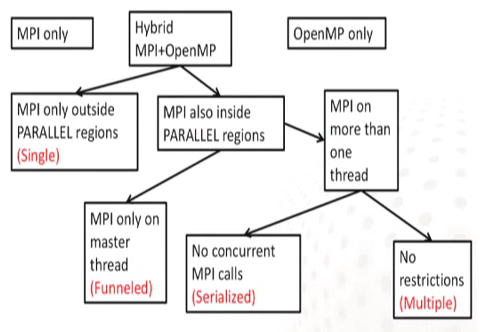
\includegraphics[width=0.5\textwidth, height=0.3\textwidth]{hybridstyles.png}
  \caption{Hybrid programming styles}
  \label{fig:hybridstyles}
\end{figure}

\subsubsection{Benefits}

\textbf{Load balancing} is hard to achieve as the number of processes increases.
With the hybrid approach, we have less processes and can dynamically changes the
number of threads per process which can improve the load balance. OpenMP also
provides the capability to perform dynamic load balancing. \\

\noindent \textbf{Reduced messages} is observed as direct memory read and write are
performed inside a node which reduces overhead caused by exchange of messages
using the MPI API. In addition, the aggregated messages become larger which
increase the throughput on inter-node communication. \\

\noindent \textbf{Overlapping communication and computation} can be achieved as master
thread handles inter-communication between nodes while other threads are
performing computation. With enough threads, the master thread can be used
purely for communication. \\

\noindent \textbf{Improve in memory usage} is seen in domain decomposition algorithm as
there are fewer data boundary points and less replicated data.In addition, cache
usage is also improved as data reside in shared cache.

\subsubsection{Evaluation}

\begin{figure}[H]
  \centering
  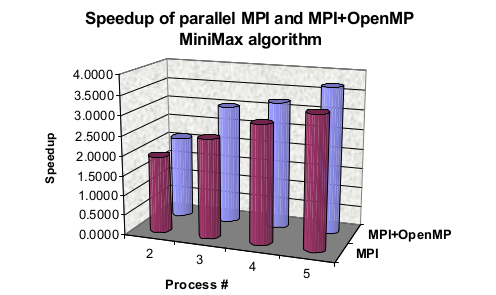
\includegraphics[width=0.6\textwidth, height=0.4\textwidth]{speedup_models.png}
  \caption{Comparing speedup using hybrid approach and pure MPI approach}
  \label{fig:speedup_models}
\end{figure}

From Figure \ref{fig:speedup_models}, the hybrid has shown to outperform the pure
approach and the increase in speedup is more significant with more processes. 

\begin{figure}[H]
  \centering
  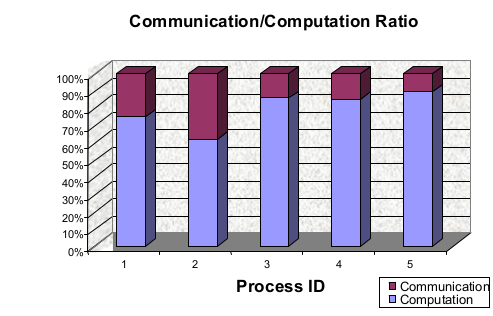
\includegraphics[width=0.4\textwidth,
  height=0.3\textwidth]{communication_ratio1.png} \hfill
  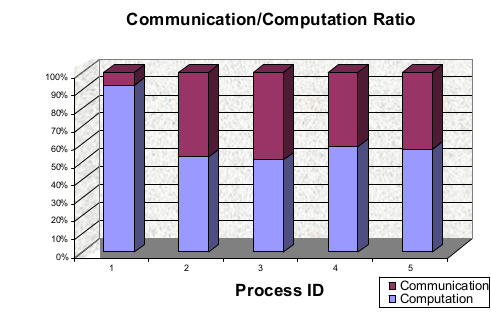
\includegraphics[width=0.4\textwidth,
  height=0.3\textwidth]{communication_ratio2.png}
  \caption{Communication/computation ratio: hybrid, pure MPI}
  \label{fig:communication_ratio}
\end{figure}

\noindent In addition, the communciation overhead with reference to Figure
\ref{fig:communication_ratio} for hybrid approach is also significantly lower
than the pure MPI implementation.


\begin{figure}[H]
  \centering
  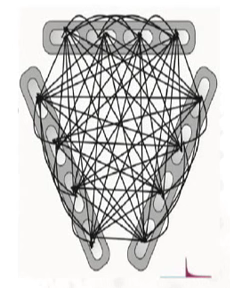
\includegraphics[width=0.4\textwidth,
  height=0.3\textwidth]{alltoall1.png} \hfill
  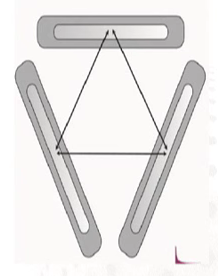
\includegraphics[width=0.4\textwidth,
  height=0.3\textwidth]{alltoall2.png}
  \caption{Benefit of hybrid programming approach}
  \label{fig:alltoall}
\end{figure}

\noindent \textbf{All-to-all communication} is often the bottleneck for parallel
algorithms as the communication overhead increases with number of processors.If
we look at Figure \ref{fig:alltoall}, the hybrid approach reduces the
communication events drastically.

\subsubsection{Disadvantages}

Compilicated programming is one of the downside of hybrid programmign styles. In
addition, creation and destruction of threads can increase overhead.

\subsection{PVS (Principle Variation Split)}

\begin{figure}[H]
  \centering
  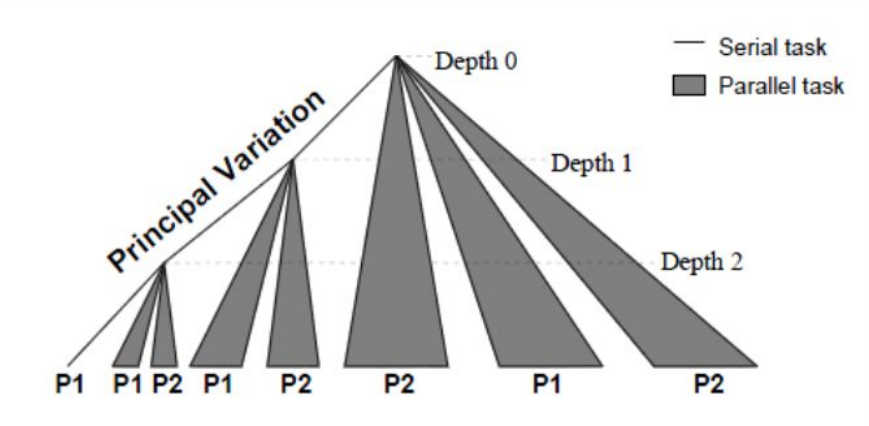
\includegraphics[width=0.5\textwidth, height=0.3\textwidth]{pvs.png}
  \caption{PV split using two processors}
  \label{fig:pvs}
\end{figure}

This approach benefits most from a strongly ordered game tree where the leftmost
child of a node is the best move. Therefore, the introduction of
\textit{transposition table} and \textit{killer heuristic} is essential.
Firstly, the PV split function is called recursively on the leftmost branch of
our tree. With the updated alpha beta bounds, regular alpha pruning is then ran
in parallel on the other children of the current node. The tree-decomposition
using PV split is shown in Figure \ref{fig:pvs}

\begin{table}[H]
\centering
\begin{tabular}{|l|l|l|}
\hline
Processors                         & Time (ms) & Speedup   \\ \hline
1                                  & 27        & -         \\ \hline
2                                  & 33        & 1.50      \\ \hline
4                                  & 18        & 2.70      \\ \hline
8                                  & 10        & 3.31      \\ \hline
8                                  & 10        & 4.73      \\ \hline
16                                 & 8.14      & 6.43      \\ \hline
32                                 & 5.7       & 5.63      \\ \hline
64                                 & 4.2       & 4.38      \\ \hline
128                                & 4.79      & 4.13      \\ \hline
256                                & 6.162     & 3.90      \\ \hline
\end{tabular}
\caption{Speedup at depth 5}
\end{table}

\begin{figure}[H]
  \centering
  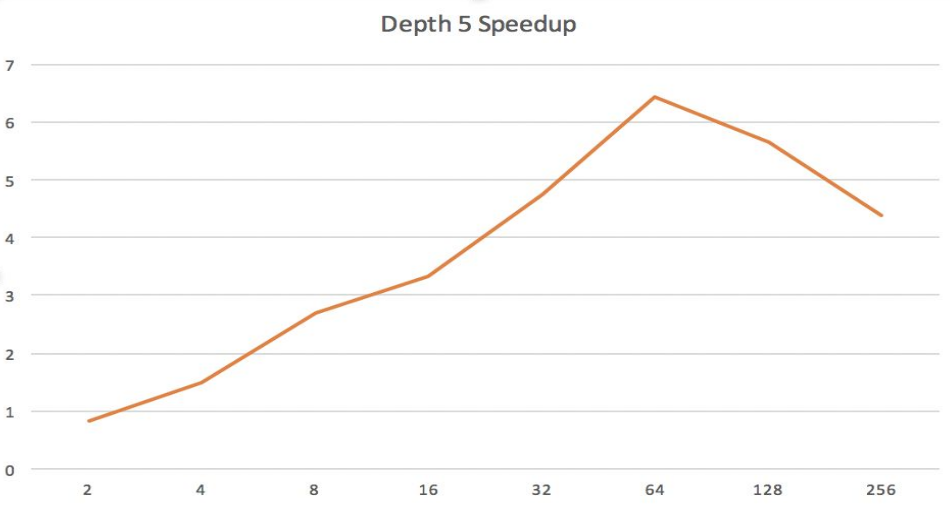
\includegraphics[width=0.6\textwidth, height=0.4\textwidth]{speedup_processor.png}
  \caption{Speedup vs processors at depth 5}
  \label{fig:speedup_processor}
\end{figure}

Looking at Figure \ref{fig:speedup_processor} of speedup against number of processors, we can observe a steady
increase in speedup with increasing processors as the number of nodes grow
exponentially with increase in depth which benefit from more parallelism. For
lower depth, the speedup decreases after certain number of processors because
the cost of communication and synchronization overshadows benefit of parallelism.

\subsection{YBWC (Young Brother Wait Concept)}

\begin{figure}[H]
  \centering
  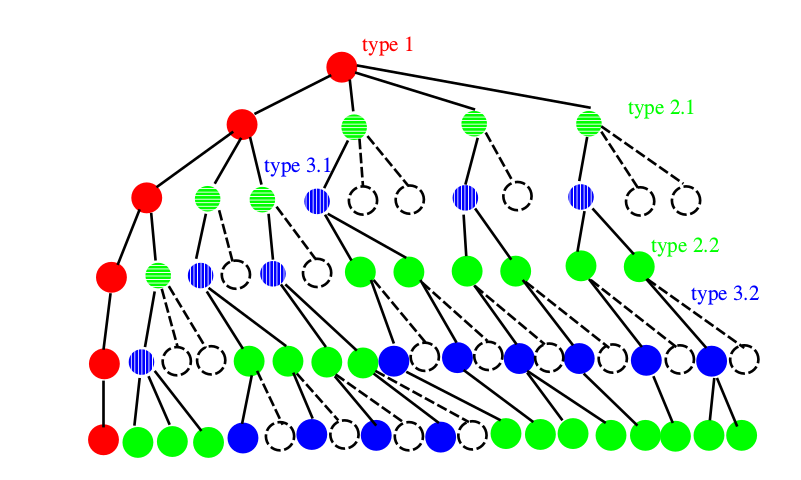
\includegraphics[width=0.6\textwidth, height=0.4\textwidth]{classification_nodes.png}
  \caption{Classification of nodes according to Knuth and Moore}
  \label{fig:classification_nodes}
\end{figure}

To achieve better parallelization for larger number of processors, we look at
Figure \ref{fig:classification_nodes} classification of nodes into 3 different
types by \cite{knuth1975analysis}. The type of node is defined according to the
rules below:

\begin{enumerate}
  \item The root of the game tree has \textbf{type-1} 
  \item The first successor of a \textbf{type-1} node has \textbf{type-1}, the
    other chilrdren have \textbf{type-2}
  \item The first successor of a \textbf{type-2} node has \textbf{type-3}, the
    other chilrdren have \textbf{type-2}
  \item All successors of a \textbf{type-3} node have \textbf{type-2} 
\end{enumerate}

\noindent To achieve better load balancing, this paper uses the variation of
YBWC \cite{feldmann1993game} that follows:

\begin{enumerate}
  \item Parallel evaluation of the successors of \textbf{type-1} node v is
    allowed only if the first son of v has been completely evaluated
  \item Parallel evaluation of the successors of \textbf{type-2} node v is
    allowed only if all the promising successors of v have been completely evaluated
  \item Parallel evaluation of the successors of a \textbf{type-3} node v is
    allowed whenever v is generated
\end{enumerate}

\noindent A promosing successor is one that is suggested by the transposition
table (best move evaluated previously) or killer heuristic.


\subsection{Better load distribution strategy}

Inspired by the work of \cite{feldmann1993game}, this paper tested the same
strategy for this project. In general, 3 stages of load distribution are
performed to achieve optimal load balancing. \\

\noindent \textbf{Local load distribution} is achieved through request for work
from a neighbour of the current idle processor. \\

\noindent \textbf{Medium range load distribution} is triggered when the
requested processor does not need any help. In this case, the request is passed
to its nearest neighbour until the request has been passed to p processors. In
this case, the requesting processor is informed of the cancellation. \\

\noindent \textbf{Global load distribution} leverages on locality of shared
transposition table and killer heuristic, master is programmed such that it
prefers processors that have previously worked with it.


%%%%%%%%%%%%%%%%%%%%%%%%%%%%%%%%%%%%%%%%%%%%%%%%%%%%%%%%%%%%%%%%%%%%%%%%%%%%%%%%%%%%%%%%%%%%%%%%%%%%

\section{Tabulation of data}

\subsection{Evaluation criteria for parallel algorithms}

$t_n(p)$ is the total time spent to evaluate position p at depth d with
processor i.

\begin{enumerate}
  \item SPE (Speedup)
    \[
      SPE(n) = \frac{\sum_{p \in P} t_1(p)}{\sum_{p \in P} t_n(p)}
    \]
  \item SO (Search Overhead), average number of nodes the parallel version
    visits more than the sequential version for a set of positions P
    \[
      SO(n) = 100 \cdot \frac{\sum_{p \in P} k_n(p)}{\sum_{p \in P} k_1(p)}
    \]
  \item LD (Processor workload), average percentage of time the processor is
    busy. $w_n(p)$ is the average amount of time a processor was busy
    \[
      LD(n) = 100 \cdot \frac{\sum_{p \in P} w_n(p)}{\sum_{p \in P} t_n(p)}
    \]
\end{enumerate}

\subsection{Speedup vs depth of tree}

\begin{figure}[H]
  \centering
  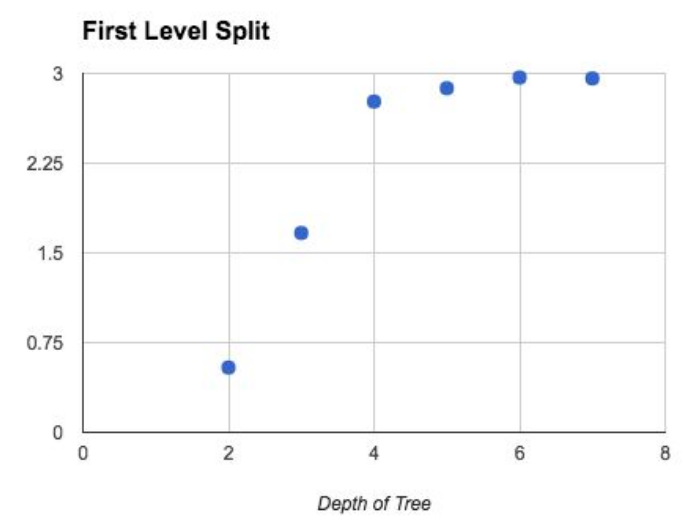
\includegraphics[width=0.6\textwidth, height=0.4\textwidth]{speedup_depthtree.png}
  \caption{Speedup vs depth of tree for level 1 split}
\end{figure}

\subsection{Per-processor elapsed time}

\begin{figure}[H]
  \centering
  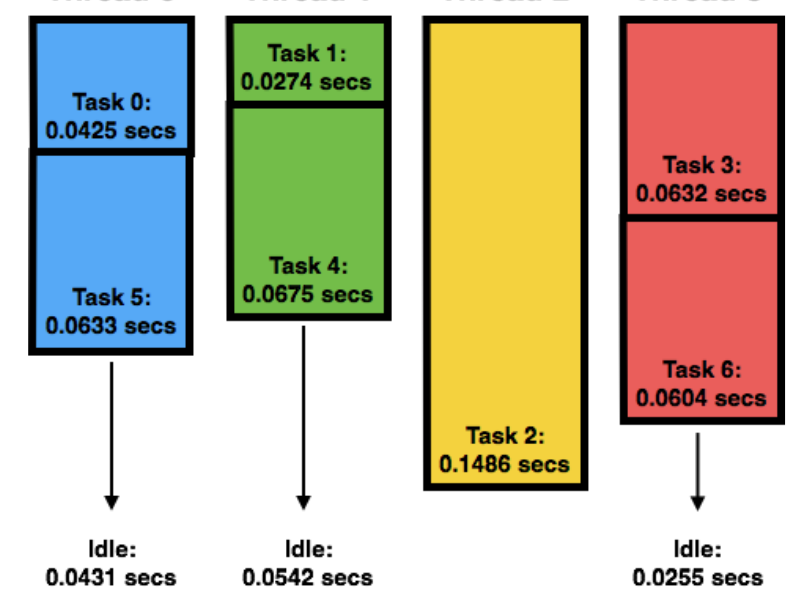
\includegraphics[width=0.6\textwidth, height=0.4\textwidth]{processor_time.png}
  \caption{Time spent by each processor}
\end{figure}

\subsection{Efficiency}

\begin{figure}[H]
  \centering
  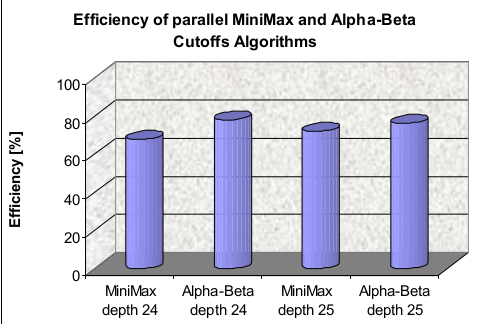
\includegraphics[width=0.6\textwidth, height=0.4\textwidth]{efficiency.png}
  \caption{Efficiency of different algorithms}
\end{figure}

\subsection{Performance of parallel algorithm}

\begin{figure}[H]
  \centering
  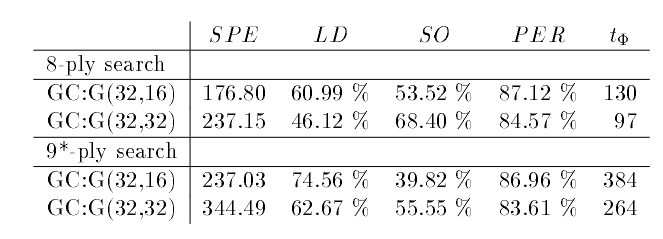
\includegraphics[width=0.6\textwidth, height=0.4\textwidth]{parallel_measure.png}
  \caption{SPE(speedup), SO(search overhead), Processor work load(LD),
    Performance per processor(PER), average run time per problem}
\end{figure}

\begin{figure}[H]
  \centering
  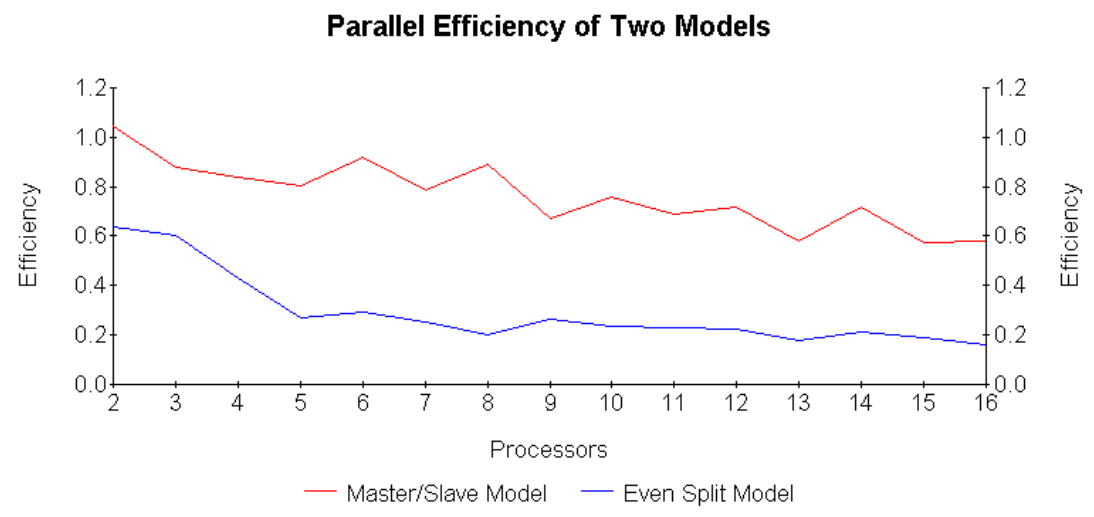
\includegraphics[width=0.6\textwidth, height=0.4\textwidth]{efficiency_model.png}
  \caption{Comparing efficiency for master-slave model and even-split model}
\end{figure}

\subsection{Nodes per second}

\begin{figure}[H]
  \centering
  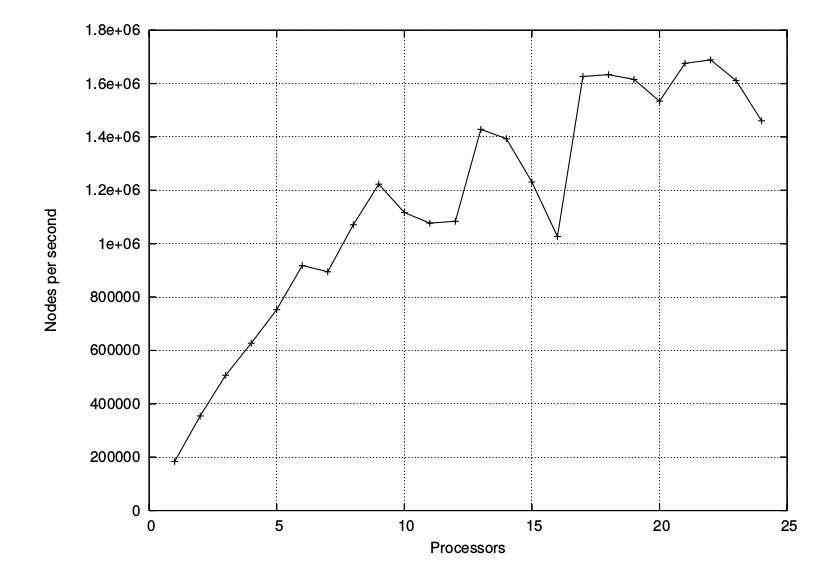
\includegraphics[width=0.6\textwidth, height=0.4\textwidth]{nps.png}
  \caption{Nodes per second (speed) for different processors}
\end{figure}

\subsection{Board size vs depth}

\begin{table}[H]
\centering
\begin{tabular}{|l|c|c|c|c|c|c|c|c|}
\hline
\multirow{2}{*}{Board dimension} & \multicolumn{8}{c|}{Depth}                                    \\ \cline{2-9} 
                                 & 1     & 2     & 3     & 4     & 5     & 6     & 7     & 8     \\ \hline
6 x 6                            & 0.596 & 0.718 & 0.429 & 0.583 & 1.278 & 0.891 & 1.588 & 2.122 \\ \hline
8 x8                             & 1.451 & 1.612 & 0.904 & 2.331 & 2.469 & 2.872 & 3.121 & 3.501 \\ \hline
10 x 10                          & 3.211 & 3.871 & 3.532 & 3.911 & -     & -     & -     & -     \\ \hline
12 x 12                          & 4.125 & 4.483 & -     & -     & -     & -     & -     & -     \\ \hline
\end{tabular}
\caption{Speedup for different board size and depth}
\end{table}

\subsection{Parallel performance of PV split}

\begin{table}[H]
\centering
\begin{tabular}{|c|c|c|c|c|c|c|}
\hline
\multirow{2}{*}{Processors} & \multicolumn{2}{c|}{Speedup} & \multicolumn{2}{c|}{Search overhead \%} & \multicolumn{2}{c|}{Time idle \%} \\ \cline{2-7} 
                            & Average & Standard deviation & Average       & Standard deviation      & Average    & Standard deviation   \\ \hline
2                           & 1.48    & 0.325              & 8.73          & 17.4                    & 12.8       & 4.90                 \\ \hline
4                           & 2.03    & 0.546              & 24.3          & 26.3                    & 30.8       & 8.17                 \\ \hline
8                           & 2.71    & 0.803              & 46.4          & 46.3                    & 48.8       & 7.74                 \\ \hline
16                          & 2.91    & 1.07               & 83.5          & 63.5                    & 67.1       & 7.00                 \\ \hline
32                          & 3.23    & 1.21               & 94.1          & 72.5                    & 74.2       & 6.81                 \\ \hline
64                          & 4.21    & 1.45               & 115.4         & 81.2                    & 80.1       & 8.21                 \\ \hline
\end{tabular}
\caption{Parallel performance measure of PV split}
\end{table}

\begin{figure}[H]
  \centering
  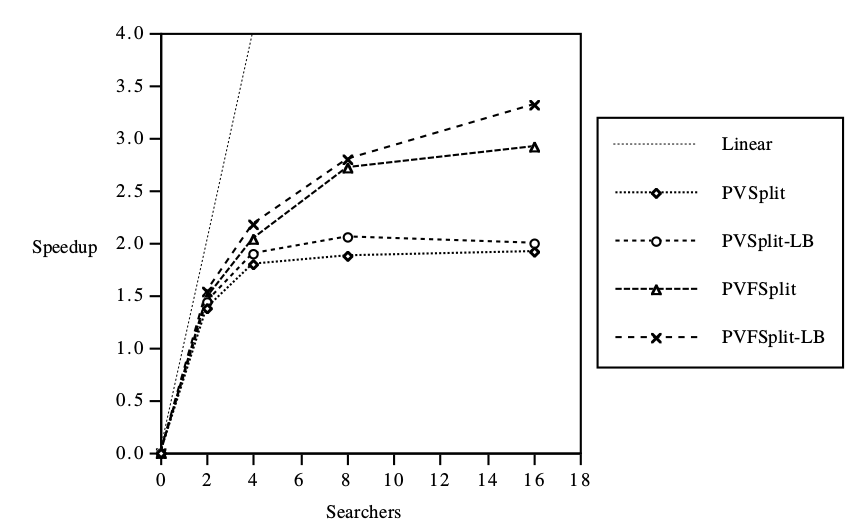
\includegraphics[width=0.6\textwidth, height=0.4\textwidth]{summary_algorithms.png}
  \caption{Summary of different parallel algorithms}
\end{figure}

%%%%%%%%%%%%%%%%%%%%%%%%%%%%%%%%%%%%%%%%%%%%%%%%%%%%%%%%%%%%%%%%%%%%%%%%%%%%%%%%%%%%%%%%%%%%%%%%%%%%

\section{Discussion}

\subsection{Split model}

The result has shown that a master-slave model provides better speedup than the
even-split model solving an othello game. The rationale is that master-slave
relationship can full use of every processors as processor that has completed
can request for more work from the master process.

\subsection{Hybrid vs Pure MPI}

The impact of hybrid programming is very relevant for our game because the
number of nodes grow exponentially with increasing depth which will increase the
communciation overhead incurred in message passing. Taking advantage of shared
memory's data locality, launching threads in MPI task can help reduce the number
of processes.

\subsection{Comparison of parallel search}

Judging from empirical results, \textbf{PV split} achieves considerable speedup for a
deep game tree and best-move ordering. However, \textbf{YBWC} manages to achieve even
better speedup when coupled with the Helpful Master concepty where a master that
has nothing to do can help one of the slave node in evaluating a subproblem. In
addition, a lockless distributed transposition table also to reduce the
synchronization overhead compared to when using a fine-grained locking mechanism.

%%%%%%%%%%%%%%%%%%%%%%%%%%%%%%%%%%%%%%%%%%%%%%%%%%%%%%%%%%%%%%%%%%%%%%%%%%%%%%%%%%%%%%%%%%%%%%%%%%%%

\bibliographystyle{acm}
\bibliography{ref}
\end{document}